\subsubsection{Login}
\subsubsection{Registration}
\subsubsection{Location Search}
The search service, is used to search and load any place in the world. As shown in the figure below, you need to click in the search box and start typing the name of the place you are searching for. \\[0.5cm]
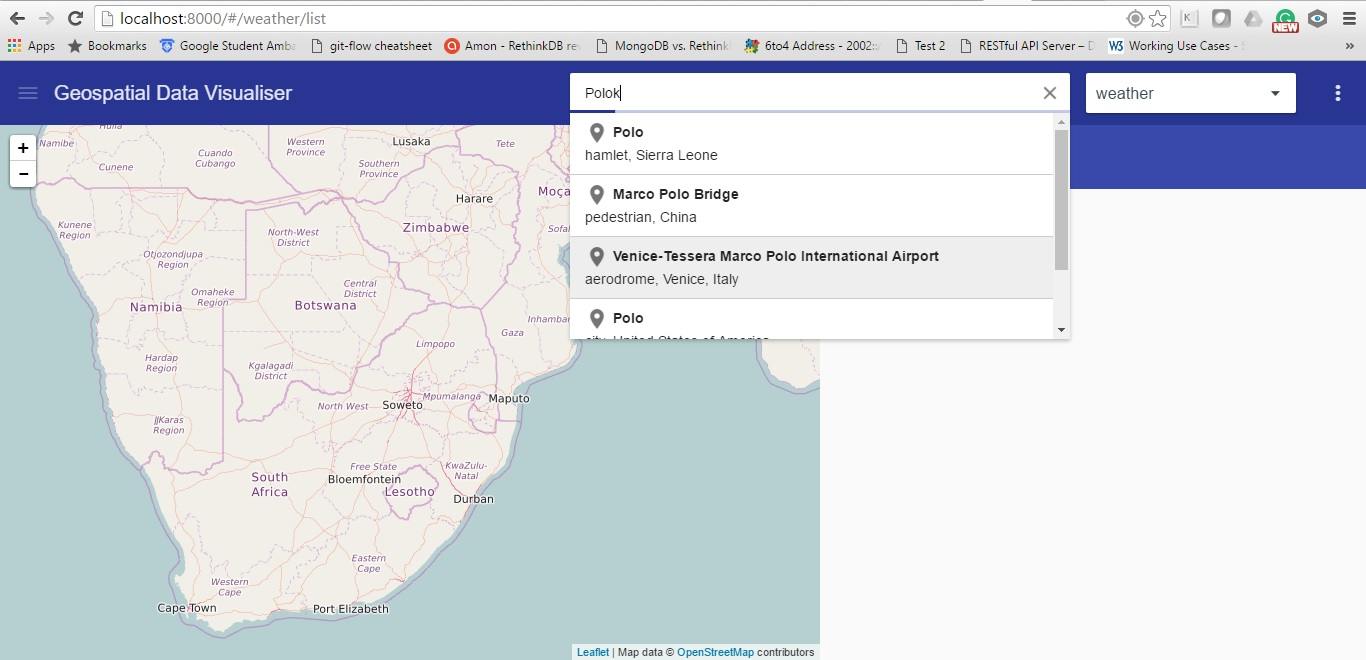
\includegraphics[width=\textwidth]{searchFunction} \\[0.5cm]
While searching a possible list of places will be loaded in a dropdown list as shown in the figure above. Once you have found the place you are looking for, use your mouse to point to the name of the place and click on that name, which will then activate a process of reloading the map to the place you have selected, like the figure shown below. A marker will be placed to show the location you queried. \\[0.5cm]
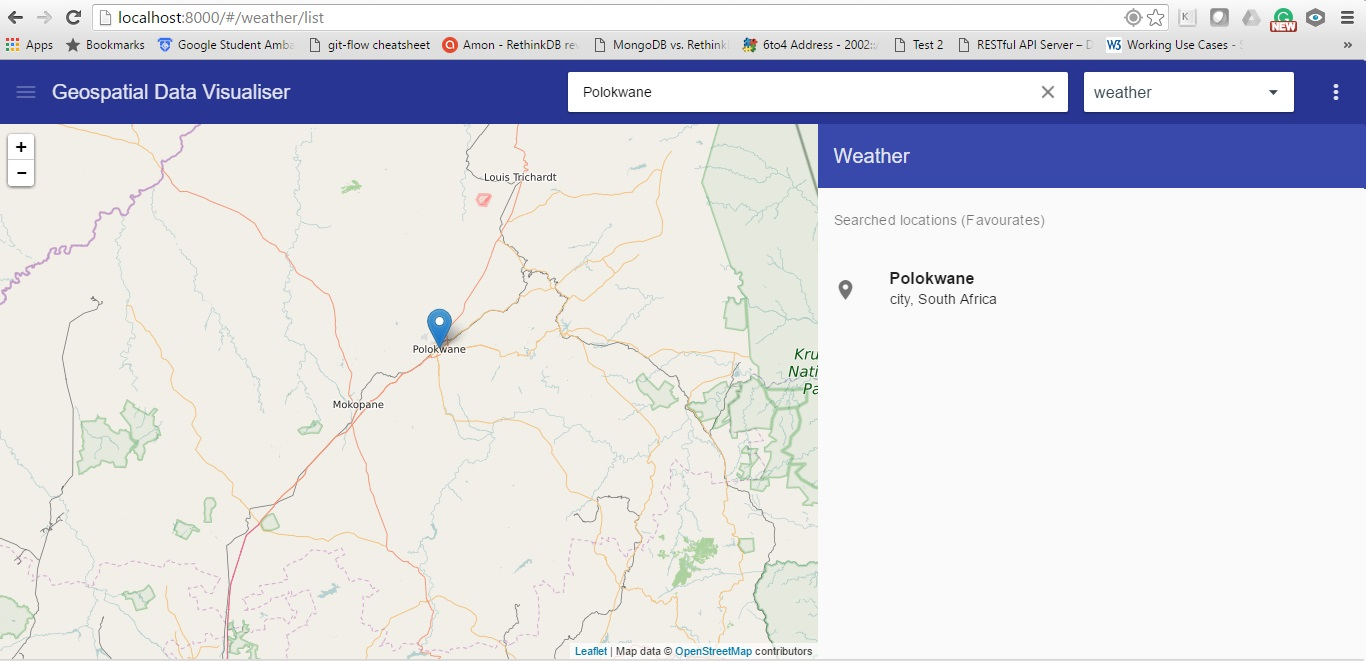
\includegraphics[width=\textwidth]{searchResult} \\[0.5cm]
The search feature is also linked to other functions of the site. When the weather center is currently active, the location name will be added to the listed of locations you have already searched for as shown above. These features will be explained in more detail in sections about the respective features.
\subsubsection{Disaster Center}
\subsubsection{Weather Center}
\subsubsection{Map Features}